\uuid{2lAA}
\exo7id{5543}
\titre{exo7 5543}
\auteur{rouget}
\organisation{exo7}
\datecreate{2010-07-15}
\isIndication{false}
\isCorrection{true}
\chapitre{Conique}
\sousChapitre{Conique}
\module{Géométrie}
\niveau{L2}
\difficulte{}

\contenu{
\texte{
\label{exo:routhe4}
Etudier les courbes dont une équation polaire (en repère orthonormé direct) est
}
\begin{enumerate}
    \item \question{$r=\frac{1}{1+2\cos\theta}$,}
\reponse{$\mathcal{C}$ est une conique d'excentricité $2$ et donc une hyperbole.

$$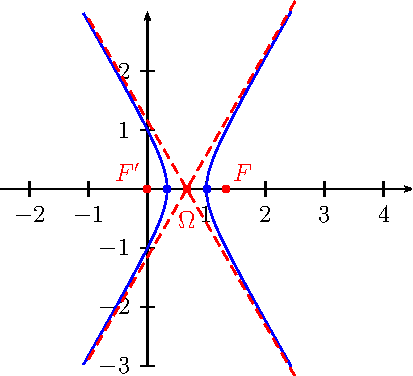
\includegraphics{../images/pdf/2lAA-1.pdf}$$

L'axe focal est $(Ox)$. Les sommets sont les points d'intersection de $\mathcal{C}$ et $(Ox)$ c'est-à-dire les points $M(0)$ et $M(\pi)$ de coordonnées cartésiennes respectives $A'\left(\frac{1}{3},0\right)$ et $A(1,0)$. Le centre $\Omega$ est le milieu de $[AA']$ c'est-à-dire $\Omega\left(\frac{2}{3},0\right)$.
L'un des foyers est $F'=O$ et l'autre est le symétrique de $F'$ par rapport à $\Omega$ : c'est le point $F\left(\frac{4}{3},0\right)$. Puisque $a=\frac{1}{3}$ et $e=2$, les directrices sont les droites d'équation $x=x_\Omega-\frac{a}{e}=\frac{1}{2}$ et $x=\frac{5}{6}$.
Les branches infinies sont obtenues pour $\theta=\pm\frac{2\pi}{3}$. Les asymptotes sont donc les droites passant par $\Omega$ d'angle polaire $\pm\frac{2\pi}{3}$. Ce sont les droites d'équations cartésiennes $y=\pm\sqrt{3}\left(x-\frac{2}{3}\right)$.}
    \item \question{$r=\frac{1}{1+\cos\theta}$,}
\reponse{$\mathcal{C}$ est une conique d'excentricité $1$ et donc une parabole.

$$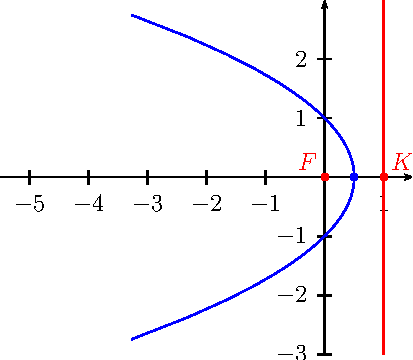
\includegraphics{../images/pdf/2lAA-2.pdf}$$

L'axe focal est $(Ox)$. Le sommet est le point $M(0)$ de coordonnées cartésiennes $S\left(\frac{1}{2},0\right)$.
Le foyer est $F=O$. Le point $K$ est le symétrique de $F$ par rapport à $S$ et a pour coordonnées $(1,0)$. La directrice a donc pour équation $x=1$.}
    \item \question{$r=\frac{1}{2+\cos\theta}$,}
\reponse{$\mathcal{C}$ est une conique d'excentricité $e=\frac{1}{2}$ et donc une ellipse.

$$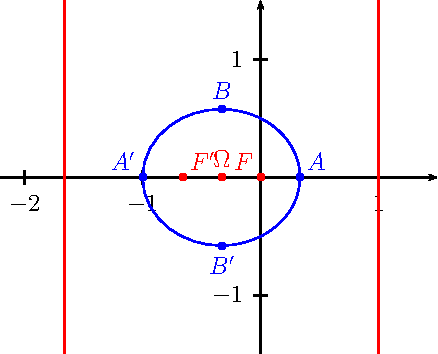
\includegraphics{../images/pdf/2lAA-3.pdf}$$

L'axe focal est $(Ox)$. Les sommets sur cet axe sont $A=M(0)$ de coordonnées $\left(\frac{1}{3},0\right)$ et $A'=M(\pi)$ de coordonnées $\left(-1,0\right)$. Le centre $\Omega$ est le milieu de $[AA']$ et a pour coordonnées $\left(-\frac{1}{3},0\right)$.
L'un des foyers est $F=O$. L'autre est le symétrique de $F$ par rapport à $\Omega$ : c'est le point $F'$ de coordonnées $\left(-\frac{2}{3},0\right)$. Par suite, $c=\frac{1}{3}$ $b=\sqrt{a^2-c^2}=\sqrt{\left(\frac{2}{3}\right)^2-\left(\frac{1}{3}\right)^2}=\frac{1}{\sqrt{3}}$. D'où les sommets $B\left(-\frac{1}{3},\frac{1}{\sqrt{3}}\right)$ et $B'\left(-\frac{1}{3},-\frac{1}{\sqrt{3}}\right)$.
Les directrices sont les droites d'équations $x=x_\Omega+\frac{a}{e}=1$ et $x=-\frac{5}{3}$.}
    \item \question{$r=\frac{1}{1-\sin\theta}$,}
\reponse{$M\left(\theta-\frac{\pi}{2}\right)=\left[r\left(\theta-\frac{\pi}{2}\right),\theta-\frac{\pi}{2}\right]=\left[\frac{1}{1+\cos\theta},\theta-\frac{\pi}{2}\right]=\text{rot}_{O,-\pi/2}\left(\left[\frac{1}{1+\cos\theta},\theta\right]\right)$. Donc $\mathcal{C}$ est l'image de la parabole d'équation polaire $r=\frac{1}{1+\cos\theta}$ par le quart de tour indirect de centre $O$.

$$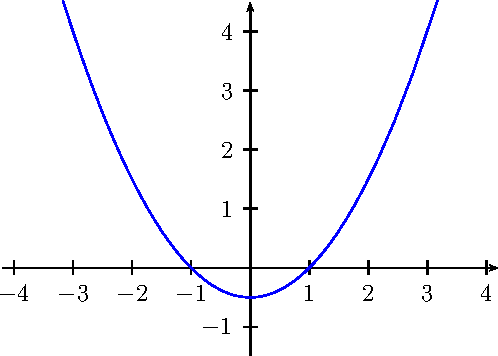
\includegraphics{../images/pdf/2lAA-4.pdf}$$}
    \item \question{$r=\frac{1}{2-\cos\theta}$.}
\reponse{$M\left(\theta+\pi\right)=\left[r\left(\theta+\pi\right),\theta+\pi\right]=\left[\frac{1}{2+\cos\theta},\theta+\pi\right]=s_O\left(\left[\frac{1}{2+\cos\theta},\theta\right]\right)$. Donc $\mathcal{C}$ est l'image de l'ellipse d'équation polaire $r=\frac{1}{2+\cos\theta}$ par la symétrie centrale de centre $O$.

$$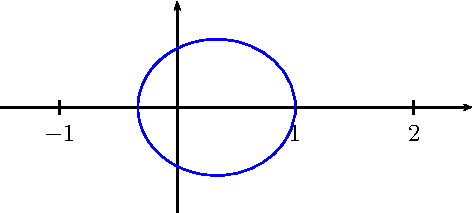
\includegraphics{../images/pdf/2lAA-5.pdf}$$}
\end{enumerate}
}
